\documentclass[sigconf]{acmart}
\settopmatter{printacmref=false} % Removes citation information below abstract
\renewcommand\footnotetextcopyrightpermission[1]{} % removes footnote with conference information in first column
\pagestyle{plain} % removes running headers

\usepackage[utf8]{inputenc}
\usepackage{caption,subcaption}

\title{CPSC 4910 Capstone Project: DeepGreen Final Report}
\author{Jesse Brown, Cameron Ogle, Charles Ritter, Bennett Cooper, Justin McCabe}

\usepackage{natbib}
\usepackage{graphicx}

\begin{document}

\maketitle

\section{Introduction}
In order to perform more complex computations in greater quantity, computer processors require an increasing amount of energy. This energy intake results in a large quantity of waste heat which must be vented away from the processor which takes again a large amount of energy. We do not know of any way to reduce the power draw of the processors themselves, but there are many methods currently in development to reduce the energy needed to draw heat away from the processors. The focus of this project was immersion cooling using Submer's SmartPod system which claims to provide equivalent or better cooling with lower power draw. It also does not have the common drawback of immersion cooling solutions that the computing hardware does not have its operation become severely impeded if it should ever leave the coolant.
\\\\
The goal of this project is to lay the foundation for future work which seeks to compare the performance of high-performance servers under advanced load while under conventional air cooling versus Submer's immersion cooling solution. We hypothesize that immersing a computer in the pod will provide more powerful cooling than air cooling while also requiring less energy. Towards this goal we have developed an experiment methodology in order to ensure parity between the data collected from air-cooled servers and immersion-cooled servers as well as collected preliminary data from air-cooled servers which will be compared against immersion-cooled servers. This included developing a computing cluster which was used to manage the servers, selecting benchmarks, implementing a system to automate testing, analyzing the results, and generating figures. Together, we have laid a strong foundation for Clemson's Scalable Computing \& Analytics lab and Submer to continue their work pushing the bounds of high-performance computing.

\section{Cluster Configuration}
The cluster is configured with one publicly accessible node acting as the gateway for the rest, which are all on the same private subnet. Each node is running Ubuntu server 18.04; the installation is done through PXE, with the gateway node providing the necessary files for installation, and automated with Kickstart. In doing so, we are able to easily add new servers to our cluster for experimentation with minimal intervention and start-up time.
\\\\
Testing the hardware thoroughly required bench-marking software that would yield useful data to our cause. Our benchmarks of choice were those that replicated real world use cases and stressed the processor to its limits. An open source tool by the name of Phoronix Test Suite met our criteria as they have a host of multi-core tests all within a simple package. Within this test suite we decided on five different benchmarks that would replicate different real world workloads while also generating useful data. The first benchmark chosen was Blender BMW render. This is a common multi-core use case of a modern processor that is perfect for demonstrating real world performance increases on cooling alterations. The next is x265 video compression; here we have another tool for compressing 1080p video using x265. The compression software uses all the cores of the CPU. Following this test we use c-ray. This small tool is a ray tracing utility focused on shading a scene with dynamic lighting and rendering polygons. This is a modern and scientific testing load with multi-core capability. Our next test is building the Linux kernel. Compilation is stressful and part of many scientific processes. This test accomplishes that while utilizing multiple cores over a long duration. Finally, the last test is john the ripper. This test stresses the CPU by performing Blowfish and MD5 hashing repeatedly. This can replicate a cryptocurrency mining protocol and provide insight as to how these CPUs perform in that environment.
\\\\
While that concludes the software we use from the Phoronix Test Suite, we use one more utility that is a native package of Ubuntu called stress-ng. This tool performs mixed operations that stress the CPU in the most demanding way we can. It does not generate an actual benchmark metric, but it does give us useful data to record what is happening when the CPU is under maximum load.
\\\\
Running these benchmarks on every node in every configuration would get incredibly time consuming and tedious if run by hand. Thus it was necessary for us to implement a task scheduling service to automate the workflow. We used a utility called Slurm for this task that synchronizes work among server nodes and prevents workloads from interfering with one another by centralizing it. This was crucial to implementing a controlled environment as every test is run at specific times with waiting intervals between them. Every test is run in order as detailed above in the phoronix benchmark section. After each test completes,  it has a cool down period of 15 minutes before running the next test. These are all run in succession until the last test, stress-ng, is finished. It follows that stress-ng was used a bit differently. Since our goal was to stress the CPU as much as possible, it was important to run the test with different amount of core utilization as all our server models differed in core/thread count. The command was run with the maximum amount of threads the processor contained and with half the amount of memory. This way we were to accomplish memory testing without adding unnecessary bottlenecks.
\begin{table}
    \centering
    \begin{tabular}{|l|l|l|}
         \hline
         \textbf{Server Model} & \textbf{CPU} & \textbf{Memory} \\ \hline
         Dell PowerEdge 1950 & Intel Xeon E5520 & 8GB DDR3 \\ \hline
         Dell PowerEdge 2950 & Intel Xeon 5150 & 32GB DDR2 \\ \hline
         Dell PowerEdge R610 & Intel Xeon E5345 & 12GB DDR2 \\ \hline
    \end{tabular}
    \caption{Basic server information}
    \label{tab:my_label}
\end{table}

\section{Methodology}
While Phoronix is able to capture hardware information while the test is running, we needed more control over it to apply it to more than just the suite itself. To consistently gather system information at any point in time, we developed a system monitoring tool that records the system temperature, CPU utilization, and memory usage. This tool was run along side each benchmark to record the system information as the benchmarks ran and was later formatted for easy analysis and visualization.
\\\\
In order to compare the effectiveness of Submer's liquid immersion cooling we want to collect metrics that represent the capability to control the operating temperature in high usage situations. In order to do this we record the temperature of our CPU as we run benchmarks that stress the CPU. By collecting the temperature during execution we are able to see if Submer's SmartPod is capable of maintaining a lower temperature than air cooling or prolong the time it takes to reach higher temperatures. We collect a large range of data in various operating configurations, namely application and frequency, to extensively compare the two environments.

\section{Results}
The data collected is collected by a monitoring tool we developed in house to monitor the CPU usage, CPU temperature, and system usage. This data is then extracted based on the start time and end time of the test being performed, the result culminates into CSV files which are then imported into R Studio for data analysis and visualization. The data cleaning process is very minimal due to the flexibility in our reporting tool, we are able to change the output into a format that is easy to interpret and work with. In the early stages it was important to understand the accuracy and precision of our monitoring, with these visualizations of the data it made it easier for us to validate aspects of program and the environment we set up.
\\\\
The other important data we collected was the temperature of the cores over the duration of the tests. To understand the effective difference in an air cooled versus a fully submerged cooling environment arguably the most important factor is heat. The monitoring tool collects the temperature of all the cores of the CPU at approximately a one second interval. Figures 1 and 2 show the recorded temperature of individual CPU cores during the execution of one of the benchmark tests.   
\begin{figure}[h]
    \centering
    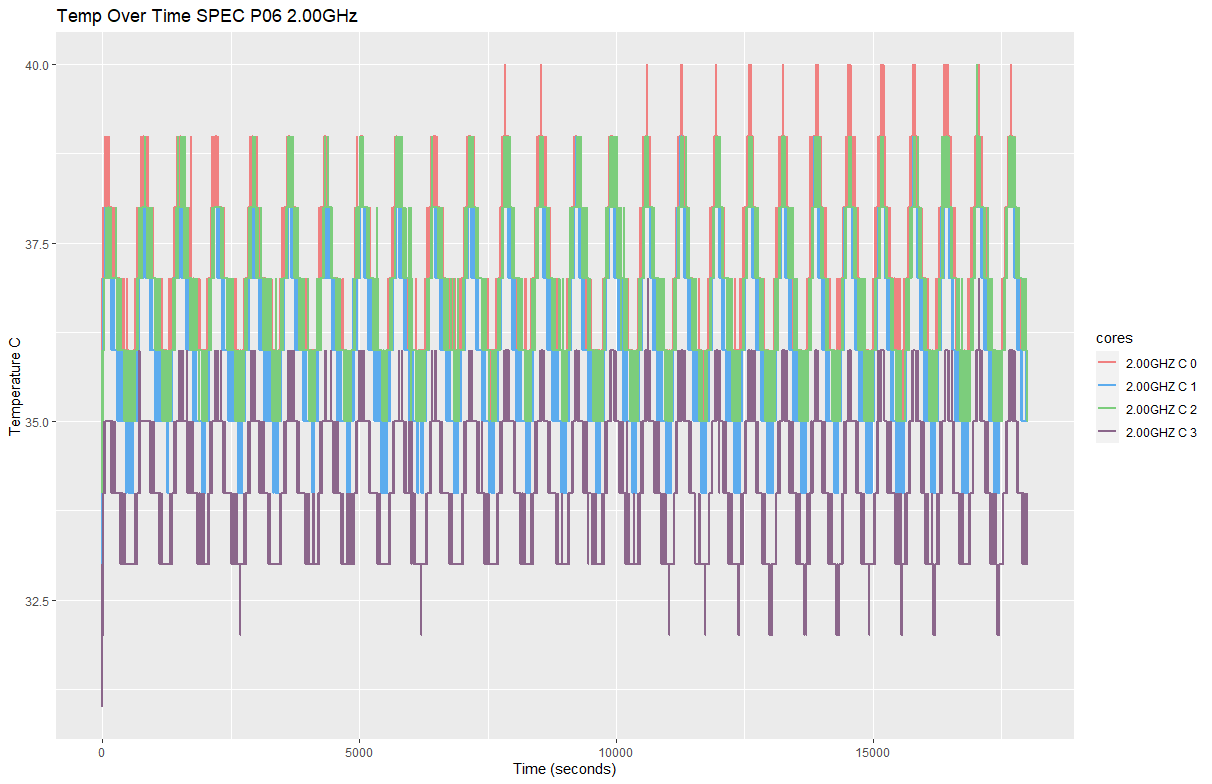
\includegraphics[scale=.27]{p06swim2ghztemp.png}
    \caption{Each line on this plot is the temperature of each core over the duration of the same test, the swim benchmark of the SPEC OMP 2012 suite, in Figure 1 at 2.00 GHz}
\end{figure}
\begin{figure}[h]
    \centering
    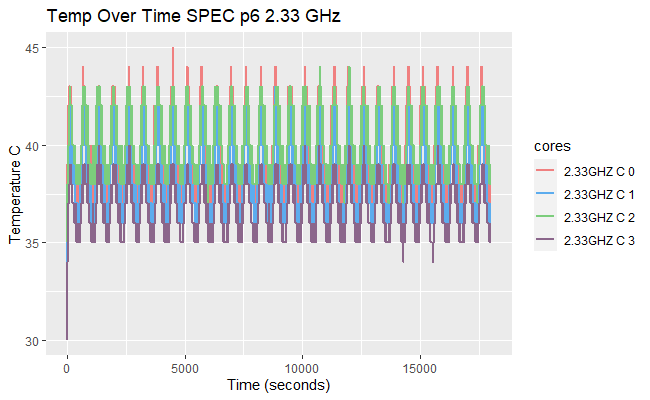
\includegraphics[scale=.55]{p06temp233ghz.png}
    \caption{Each line on this plot is the temperature of each core over the duration of the same test, the swim benchmark of the SPEC OMP 2012 suite, in Figure 1 at 2.33 GHz}
\end{figure}
\\\\
As expected, we can see from Figures 1 and 2 that the temperature of our CPU is dependent on the operating frequency. Our current results are limited to the air cooled environment and will later be used as a basis for comparing the effectiveness of cooling in Submer's SmartPod when identical tests can be run in that environment. 

\section{Limitations}
In this section we will discuss the limitations of our current setup and the impact they have on our experiments and the data that can be recorded. The majority of the limitations are due to the age of the hardware we have and the unavailability of underlying control features. As such we have limited control over certain hardware settings and inability to collect certain metrics at the desired scope.
\\\\
Due to the age of some of the hardware available, we were unable to control certain aspects of the CPUs that would help in providing more insight into power efficiency. For example, the Dell PowerEdge R610 did not support the ability to pass control of the CPU frequency to the operating system and as a result we were not able to fix the frequency on this server for our experiments. Furthermore, none of the CPUs we had for testing exposed any method for controlling, or reading, the voltage independently which limited our ability to perform our experiments at near-threshold voltages for minimal power consumption. Lastly, we have no method for collecting power consumption metrics, or even the necessary measurements to compute power, and as a result, the only meaningful metric we can collect is temperature to determine cooling efficiency. 
\\\\
One last special limitations we had during this project was a result of the time frame we worked on this; social distancing and university closure due to the COVID-19 outbreak prevented any physical access to our cluster in our air cooled environment and indefinitely suspended our access to the liquid immersion environment. As a result of these precautions, we were not able to sufficiently setup our liquid immersion environment for testing and do not have data for comparison. Moreover, without physical access to our air cooled environment we limited the intensity of our experiments to prevent any hardware failures that would result in losing access to our cluster until physical access could be permitted. 

\section{Future Work}
Future work on this project will primarily come as a result of resolving the limitations mentioned above. Further work can be done by enabling the collection of power consumption data allowing direct comparison of power and cost efficiency of the two cooling methods. Getting the ability to control CPU voltage independently will also allow further experimentation at lower power levels and give insight for systems that run with near-threshold voltage. Furthermore, the extent of our current experiments is limited to CPUs but other devices, such as GPUs, FPGAs, network adapters, etc., may all perform differently from the CPU when immersed in liquid. 
\\\\
In order to compare between the two cooling environments we will also need to repeat our experiments in the Submer SmartPod when access is available for setup. This is crucial work that needs to be done as this is a compartive study between traditional air cooling and Submer's approach to liquid immersion cooling. Until the environment in the SmartPod is setup we are unable to make any meaningful conclusions regarding the advantages or disadvantages of either cooling approach. 

\section{Conclusion}
This project was done through Clemson's School of Computing's Capstone course. The Capstone course offers the opportunity for junior and senior undergraduate students to work with an actual industry client to gain experience working on a real world project. Our project was centered around exploring the benefits and drawbacks of liquid immersion cooling in a high performance computing setting compared to the traditional air cooling approach. In order to begin comparison we needed to setup a cluster of servers for that would be used for testing in both environments in a manner that would support easy additions of new hardware with minimal manual intervention.
\\\\
In our project, we have completely established the method for setting up servers in our cluster and automated the process of adding new machines as much as possible. This is important because it will allow us to add new hardware with minimal difficulty later in the project and quickly recreate our environment in the Submer SmartPod when it is available. Furthermore, we have collected preliminary results in the air cooled environment and learned the constraints of the hardware available to us. By doing so we know what is and is not possible on the current hardware we have and have a basis of comparison for cooling efficiency in our air cooled environment.
\end{document}
